\documentclass[11pt,a4paper]{article}

% ---------- Plain, no-colour packages ----------
\usepackage[margin=2.4cm]{geometry}
\usepackage[utf8]{inputenc}
\usepackage[T1]{fontenc}
\usepackage{booktabs}
\usepackage{amssymb}
\usepackage{longtable}
\usepackage{array}
\usepackage{enumitem}
\usepackage[hidelinks]{hyperref} % hidelinks = no coloured link boxes
\usepackage{titlesec}
\usepackage{fancyhdr}
\usepackage{tikz}
\usepackage{tabularx}
\usepackage{float}
\usetikzlibrary{shapes.geometric,positioning}

\setlist[itemize]{topsep=2pt,itemsep=2pt,parsep=0pt}
\setlist[enumerate]{topsep=2pt,itemsep=2pt,parsep=0pt}

\titleformat{\section}{\normalfont\Large\bfseries}{\thesection}{1em}{}
\titleformat{\subsection}{\normalfont\large\bfseries}{\thesubsection}{1em}{}
\titleformat{\subsubsection}{\normalfont\normalsize\bfseries}{\thesubsubsection}{1em}{}

\pagestyle{fancy}
\fancyhf{}
\renewcommand{\headrulewidth}{0.4pt}
\fancyhead[L]{\small Software Requirements Specification -- VFMS}
\fancyhead[R]{\small\thepage}

\newcommand{\todofill}[1]{\textit{[#1]}}

\begin{document}

% ==================== Cover Page ====================
\begin{titlepage}
\centering
\vspace*{2cm}
{\LARGE\bfseries Software Requirements Specification}\\[0.5cm]
{\Large Vehicle Fleet Management System (VFMS)}\\[2cm]

\vspace{2cm}
Submitted in Partial Fulfilment of the Requirements of\\
Software Engineering Module (CMPG224)\\
North-West University, Mafikeng
\end{titlepage}

% ==================== Project Team and Approvals ====================
\section*{Project Team and Approvals}

\begin{table}[H]
\centering
\begin{tabularx}{\textwidth}{|X|X|X|}
\hline
\textbf{Role} & \textbf{Name} & \textbf{Student Number} \\
\hline
Backend Developer & Tobo Mohlamonyane & 47812036 \\
\hline
Frontend / UX Developer & Malejane MM & 52427064 \\
\hline
Database Engineer & TJ Mnisi & 51470470 \\
\hline
Security \& DevOps Engineer / Backend Developer & Karabo Makgala & 50081659 \\
\hline
QA \& Documentation Lead / Frontend Developer & SK Ketani & 55825184 \\
\hline
\multicolumn{3}{|c|}{\textbf{Client Representative}} \\
\hline
Lecturer / Client Representative & Prof. Bassey Isong &  \\
\hline
\end{tabularx}
\end{table}

\clearpage

\tableofcontents
\newpage

% ==================== 1. Introduction ====================
\section{Introduction}

\subsection{Purpose}
This Software Requirements Specification (SRS) defines the functional and
non-functional requirements for the Vehicle Fleet Management System (VFMS).
It serves as the basis for system design and development, and as a
reference for testing and acceptance. The intended audience includes the
development team, the project supervisor, and any stakeholders involved in
the project.

\subsection{Project Scope}
Many small companies currently manage their vehicles, drivers, and vehicle
maintenance records using spreadsheets, which are easy to lose, difficult
to search, and offer no meaningful protection for sensitive information.
VFMS addresses this by giving every vehicle and driver its own digital
record, letting authorised staff quickly find the information they need,
and ensuring that only authorised users can see sensitive details such as
a driver's licence number.

Core functions include:
\begin{itemize}
  \item User authentication and role-based access control
  \item Vehicle record management (create, view, update, delete)
  \item Driver record management (create, view, update, delete)
  \item Assigning drivers to vehicles and maintaining assignment history
  \item Logging and viewing vehicle maintenance and service history
  \item Searching vehicle and driver records by relevant fields
\end{itemize}

The following are explicitly \textbf{out of scope}:
\begin{itemize}
  \item Hardware infrastructure setup (servers, networking equipment)
  \item Integration with third-party systems (e.g. payment gateways,
  biometric access systems)
  \item Large-scale production deployment or hosting infrastructure
\end{itemize}

\subsection{Definitions, Acronyms, and Abbreviations}
\begin{longtable}{@{}p{3.2cm}p{11.3cm}@{}}
\toprule
Term / Acronym & Definition \\
\midrule
\endhead
SRS & Software Requirements Specification -- this document \\
FR & Functional Requirement \\
NFR & Non-Functional Requirement \\
CRUD & Create, Read, Update, Delete -- the basic data operations \\
RBAC & Role-Based Access Control -- restricting system actions based on
a user's assigned role \\
VFMS & Vehicle Fleet Management System -- the system described by this
document \\
POPIA & Protection of Personal Information Act (Act No.\ 4 of 2013) --
South African data protection legislation applicable to systems that
store personal information, including driver details \\
\bottomrule
\end{longtable}

\subsection{References}
\begin{itemize}
  \item Sommerville, I. (2016). \textit{Software Engineering} (10th ed.).
  Pearson.
  \item CMPG 224 Information Management System Project Brief, 2026.
  \item Protection of Personal Information Act, No.\ 4 of 2013 (POPIA),
  Republic of South Africa.
\end{itemize}

% ==================== 2. Overall System Description ====================
\section{Overall System Description}

\subsection{System Context}
VFMS is a self-contained, browser-accessible system used internally by a
single organisation to manage its own vehicle fleet. It does not exchange
data with any external system: all vehicle, driver, assignment, and
maintenance data originates from, and is consumed by, authorised users of
the organisation through the system's own interface. Users interact with
the system directly; there are no automated external actors.

\subsection{Stakeholder Description}
\begin{longtable}{@{}p{3.6cm}p{5.5cm}p{5.4cm}@{}}
\toprule
Stakeholder & Role / Relationship to System & Primary Interest \\
\midrule
\endhead
Administrator & Full access; manages vehicle, driver, and maintenance
records and oversees system use & Data integrity, complete visibility,
reliable record-keeping \\
Fleet Manager & Uses the system daily to assign drivers, review
maintenance history,  & Fast search, accurate
reporting, minimal manual effort \\
Staff Member & Uses the system for day-to-day operational tasks such as
logging maintenance events & Simple interface, restricted visibility of
sensitive driver information \\
Driver (indirect) & Does not use the system directly, but their personal
information (licence number, expiry date) is stored and processed by it
& Their personal information is kept secure and used only for its
intended fleet-management purpose \\
\bottomrule
\end{longtable}

\subsection{Assumptions and Dependencies}
\textbf{Assumptions:}
\begin{itemize}
  \item Users have basic computer literacy and access to a web browser.
  \item The system will be hosted on infrastructure accessible to all
  authorised users over the internet.
  \item Each user is assigned exactly one role (Administrator, Manager, or
  Staff) at any given time.
\end{itemize}

\textbf{Dependencies:}
\begin{itemize}
  \item The system requires a relational database to persist vehicle,
  driver, assignment, and maintenance records.
  \item The system requires a functioning network connection between the
  client and server for all operations.
  \item The chosen technology stack is available and functional on the
  development and deployment environments.
\end{itemize}

% ==================== 3. Functional Requirements ====================
\section{Functional Requirements}

\subsection{User Authentication and Access Control}
\begin{longtable}{@{}p{1.3cm}p{9.2cm}p{1.6cm}p{2.4cm}@{}}
\toprule
ID & Requirement & Priority & Source \\
\midrule
\endhead
FR01 & The system shall require a user to log in with a username and
password before accessing any vehicle, driver, or maintenance data. &
High & Stakeholder interview \\
FR02 & The system shall enforce role-based access control with at least
three roles: Administrator, Manager, and Staff. & High & Stakeholder
interview \\
FR03 & The system shall restrict access to a driver's licence number to
users with the Administrator or Manager role. & High & Stakeholder
interview \\
FR04 & The system shall store user passwords in a hashed, non-reversible
format and shall never store or transmit a password in plain text. &
High & Security requirement \\
\bottomrule
\end{longtable}

\subsection{Vehicle Management}
\begin{longtable}{@{}p{1.3cm}p{9.2cm}p{1.6cm}p{2.4cm}@{}}
\toprule
ID & Requirement & Priority & Source \\
\midrule
\endhead
FR05 & The system shall allow an authorised user to add a new vehicle
record, capturing at minimum: registration number, make, model, year,
and status. & High & Stakeholder interview \\
FR06 & The system shall allow an authorised user to view a list of all
vehicles and the details of an individual vehicle. & High & Stakeholder
interview \\
FR07 & The system shall allow an authorised user to update the details of
an existing vehicle record. & High & Stakeholder interview \\
FR08 & The system shall allow an authorised user to remove a vehicle
record from the system. & Medium & Stakeholder interview \\
FR09 & The system shall prevent two vehicle records from being created
with the same registration number. & High & Stakeholder interview \\
\bottomrule
\end{longtable}

\subsection{Driver Management}
\begin{longtable}{@{}p{1.3cm}p{9.2cm}p{1.6cm}p{2.4cm}@{}}
\toprule
ID & Requirement & Priority & Source \\
\midrule
\endhead
FR10 & The system shall allow an authorised user to add a new driver
record, capturing at minimum: name, licence number, and licence expiry
date. & High & Stakeholder interview \\
FR11 & The system shall allow an authorised user to view a list of all
drivers and the details of an individual driver. & High & Stakeholder
interview \\
FR12 & The system shall allow an authorised user to update the details of
an existing driver record. & High & Stakeholder interview \\
FR13 & The system shall allow an authorised user to remove a driver
record from the system. & Medium & Stakeholder interview \\
FR14 & The system shall prevent two driver records from being created
with the same licence number. & High & Stakeholder interview \\
\bottomrule
\end{longtable}

\subsection{Driver-Vehicle Assignment}
\begin{longtable}{@{}p{1.3cm}p{9.2cm}p{1.6cm}p{2.4cm}@{}}
\toprule
ID & Requirement & Priority & Source \\
\midrule
\endhead
FR15 & The system shall allow an authorised user to assign a driver to a
specific vehicle. & High & Stakeholder interview \\
FR16 & The system shall maintain a history of past driver-vehicle
assignments, including the date a driver was assigned and unassigned. &
High & Stakeholder interview \\
FR17 & The system shall prevent a driver or vehicle from being assigned
if it does not already exist in the system. & Medium & Stakeholder
interview \\
\bottomrule
\end{longtable}

\subsection{Maintenance and Service History}
\begin{longtable}{@{}p{1.3cm}p{9.2cm}p{1.6cm}p{2.4cm}@{}}
\toprule
ID & Requirement & Priority & Source \\
\midrule
\endhead
FR18 & The system shall allow an authorised user to log a maintenance or
service event for a vehicle, capturing at minimum: date, cost, and
description. & High & Stakeholder interview \\
FR19 & The system shall allow an authorised user to view the maintenance
history of a specific vehicle. & High & Stakeholder interview \\
FR20 & The system shall notify an authorised user when a driver's licence
is approaching its expiry date. & Medium & Stakeholder interview \\
\bottomrule
\end{longtable}

\subsection{Search}
\begin{longtable}{@{}p{1.3cm}p{9.2cm}p{1.6cm}p{2.4cm}@{}}
\toprule
ID & Requirement & Priority & Source \\
\midrule
\endhead
FR21 & The system shall allow an authorised user to search for vehicle
records by at least registration number, make, and model. & High &
Stakeholder interview \\
FR22 & The system shall allow an authorised user to search for driver
records by at least name and licence number. & High & Stakeholder
interview \\
\bottomrule
\end{longtable}

% ==================== 4. Non-Functional Requirements ====================
\section{Non-Functional Requirements}

\begin{longtable}{@{}p{1.3cm}p{2.4cm}p{5.2cm}p{5.6cm}@{}}
\toprule
ID & Quality Attribute & Requirement & Measurement Criterion \\
\midrule
\endhead
NFR01 & Performance & The system shall return search results and record
details within an acceptable response time. & Search results and record
details must be displayed within 3 seconds under normal operating
conditions. \\
NFR02 & Scalability & The system shall accommodate growing numbers of
users and records. & The system shall support at least 20 concurrent
users and allow the addition of thousands of vehicle and driver records
over time without requiring a database redesign. \\
NFR03 & Security -- Authentication & The system shall protect stored user
passwords. & Passwords must be stored using a one-way, industry-standard
hashing algorithm. Plain-text passwords must never be stored or
transmitted. \\
NFR04 & Security -- Authorisation & The system shall restrict sensitive
driver information to permitted roles. & A user with the Staff role must
never receive a driver's licence number in any system response,
verified by automated testing. \\
NFR05 & Security -- Data Protection & The system shall protect data in
transit between client and server. & All communication between the
browser and the server must use HTTPS/TLS; no sensitive data may be
transmitted unencrypted. \\
NFR06 & Security -- Session Management & The system shall limit exposure
from unattended, logged-in sessions. & A user session shall be
automatically invalidated after 20 minutes of inactivity. \\
NFR07 & Usability & The system shall be usable without formal training.
& A user with basic computer literacy shall be able to complete a core
task (e.g.\ adding a vehicle record) within 10 minutes of first use. \\
NFR08 & Usability -- Responsiveness & The system's interface shall adapt
to common screen sizes. & The interface must remain fully functional on
desktop, tablet, and mobile screen widths, verified by manual testing on
at least three device classes. \\
NFR09 & Usability -- Error Handling & The system shall present
user-friendly error messages. & 100\% of user-facing error messages must
use plain language; no raw technical error codes may be shown to the
user. \\
NFR10 & Reliability -- Uptime & The system shall be available during
business hours. & The system shall maintain at least 99.5\% uptime during
defined business hours, measured over a rolling 30-day period. \\
NFR11 & Reliability -- Data Integrity & The system shall protect against
data loss. & The system's database shall be backed up at least once
daily, and no committed transaction may be lost in the event of a
system crash. \\
NFR12 & Maintainability & The system shall be organised for ease of
future modification. & The system shall be structured into
independently modifiable layers (e.g.\ presentation, business logic,
data access) such that a change to one layer does not require changes to
unrelated layers, verified by code review. \\
NFR13 & Legal Compliance & The system shall handle driver personal
information in accordance with applicable law. & All storage and
processing of driver personal information must comply with the
Protection of Personal Information Act (POPIA), verified against a
compliance checklist prior to deployment. \\
\bottomrule
\end{longtable}

% ==================== 5. Use Cases ====================
\section{Use Cases}

\subsection{Use Case Diagram}

\begin{center}
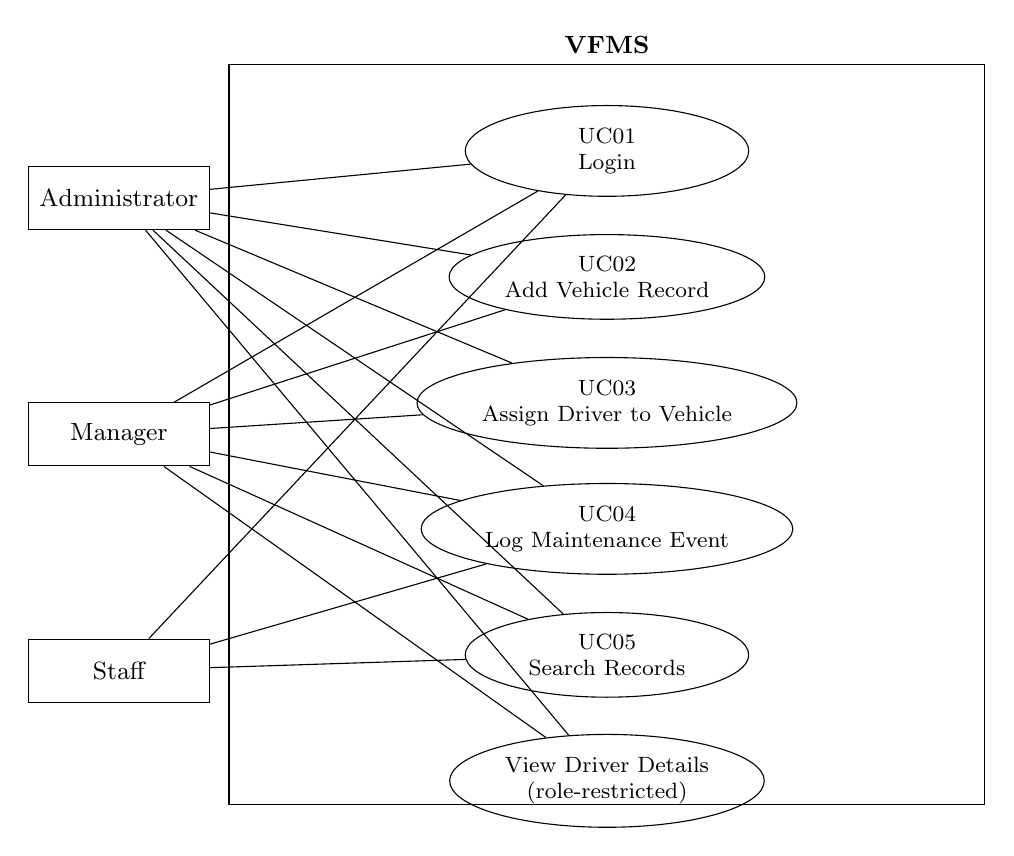
\begin{tikzpicture}[
  actor/.style={draw,minimum width=2.3cm,minimum height=0.8cm,align=center,font=\small},
  uc/.style={draw,ellipse,minimum width=3.6cm,minimum height=1cm,align=center,font=\footnotesize},
  every path/.style={thin}
]
  % Actors
  \node[actor] (admin) at (0,7) {Administrator};
  \node[actor] (manager) at (0,4) {Manager};
  \node[actor] (staff) at (0,1) {Staff};

  % System boundary
  \node[draw,minimum width=9.6cm,minimum height=9.4cm,label={[font=\small\bfseries]above:VFMS}] (boundary) at (6.2,4) {};

  % Use cases -- generous vertical spacing, single column to avoid crossing
  \node[uc] (login)      at (6.2,7.6) {UC01\\Login};
  \node[uc] (addveh)     at (6.2,6.0) {UC02\\Add Vehicle Record};
  \node[uc] (assign)     at (6.2,4.4) {UC03\\Assign Driver to Vehicle};
  \node[uc] (maint)      at (6.2,2.8) {UC04\\Log Maintenance Event};
  \node[uc] (search)     at (6.2,1.2) {UC05\\Search Records};
  \node[uc] (viewdriver) at (6.2,-0.4) {View Driver Details\\(role-restricted)};

  % Admin: all use cases
  \foreach \uc in {login,addveh,assign,maint,search,viewdriver}{
    \draw (admin) -- (\uc);
  }
  % Manager: all use cases
  \foreach \uc in {login,addveh,assign,maint,search,viewdriver}{
    \draw (manager) -- (\uc);
  }
  % Staff: login, maintenance, search only
  \draw (staff) -- (login);
  \draw (staff) -- (maint);
  \draw (staff) -- (search);
\end{tikzpicture}
\end{center}

Note: the Staff actor is deliberately not connected to \textit{View Driver
Details (role-restricted)}, reflecting FR03 -- a Staff user may search for
and view a driver record, but the licence number field is withheld.

\subsection{Use Case Descriptions}

\subsubsection*{UC01 -- User Login}
\begin{longtable}{@{}p{3.2cm}p{11.3cm}@{}}
\toprule
Field & Description \\
\midrule
\endhead
Use Case ID & UC01 \\
Related Requirements & FR01, FR02, FR04 \\
Primary Actor & Any registered user (Administrator, Manager, or Staff) \\
Preconditions & The user has a valid account. The system is running and
accessible. \\
Main Success Scenario &
1.\ User navigates to the login page.\newline
2.\ User enters username and password.\newline
3.\ System validates the credentials against the stored (hashed) password.\newline
4.\ System grants access and directs the user to the dashboard appropriate
to their role.\newline
5.\ System starts a 20-minute inactivity timer. \\
Alternative Flow 1 & 3a.\ Invalid credentials entered $\rightarrow$
system displays ``Incorrect username or password'' without indicating
which field was wrong. \\
Alternative Flow 2 & 5a.\ Session reaches 20 minutes of inactivity
$\rightarrow$ system automatically logs the user out and requires
re-authentication. \\
Postconditions & User is authenticated and an active session is
established. \\
\bottomrule
\end{longtable}

\subsubsection*{UC02 -- Add Vehicle Record}
\begin{longtable}{@{}p{3.2cm}p{11.3cm}@{}}
\toprule
Field & Description \\
\midrule
\endhead
Use Case ID & UC02 \\
Related Requirements & FR05, FR09 \\
Primary Actor & Administrator or Manager \\
Preconditions & User is logged in with a role permitted to create
vehicle records. \\
Main Success Scenario &
1.\ User selects ``Add Vehicle''.\newline
2.\ User enters registration number, make, model, year, and status.\newline
3.\ System validates that the registration number is not already in
use.\newline
4.\ System saves the new vehicle record.\newline
5.\ System confirms the record was created and displays it in the
vehicle list. \\
Alternative Flow 1 & 3a.\ Registration number already exists
$\rightarrow$ system rejects the submission and displays ``A vehicle
with this registration number already exists.'' \\
Postconditions & A new vehicle record exists in the system. \\
\bottomrule
\end{longtable}

\subsubsection*{UC03 -- Assign Driver to Vehicle}
\begin{longtable}{@{}p{3.2cm}p{11.3cm}@{}}
\toprule
Field & Description \\
\midrule
\endhead
Use Case ID & UC03 \\
Related Requirements & FR15, FR16, FR17 \\
Primary Actor & Administrator or Manager \\
Preconditions & Both the driver and the vehicle already exist in the
system. The vehicle does not currently have an active driver assigned. \\
Main Success Scenario &
1.\ User selects a vehicle and chooses ``Assign Driver''.\newline
2.\ User selects a driver from the list of existing drivers.\newline
3.\ System confirms both records exist and the vehicle has no current
assignment.\newline
4.\ System creates the assignment and records the date.\newline
5.\ System updates the vehicle's record to reflect the assigned driver. \\
Alternative Flow 1 & 3a.\ Selected vehicle already has an active driver
$\rightarrow$ system rejects the request and displays ``This vehicle
already has an assigned driver.'' \\
Alternative Flow 2 & 3b.\ Selected driver or vehicle no longer exists
$\rightarrow$ system displays ``Record not found'' and cancels the
action. \\
Postconditions & The driver is linked to the vehicle, and the assignment
is recorded in the assignment history. \\
\bottomrule
\end{longtable}

\subsubsection*{UC04 -- Log Maintenance Event}
\begin{longtable}{@{}p{3.2cm}p{11.3cm}@{}}
\toprule
Field & Description \\
\midrule
\endhead
Use Case ID & UC04 \\
Related Requirements & FR18, FR19 \\
Primary Actor & Administrator, Manager, or Staff \\
Preconditions & The vehicle already exists in the system. User is
logged in. \\
Main Success Scenario &
1.\ User selects a vehicle and chooses ``Log Maintenance''.\newline
2.\ User enters the service date, cost, and description.\newline
3.\ System validates the vehicle exists and the entered data is
complete.\newline
4.\ System saves the maintenance record.\newline
5.\ System displays the updated maintenance history for that vehicle. \\
Alternative Flow 1 & 3a.\ Required field missing $\rightarrow$ system
displays which field is missing and does not save the record. \\
Postconditions & A new maintenance record exists and is linked to the
vehicle. \\
\bottomrule
\end{longtable}

\subsubsection*{UC05 -- Search Vehicle or Driver Records}
\begin{longtable}{@{}p{3.2cm}p{11.3cm}@{}}
\toprule
Field & Description \\
\midrule
\endhead
Use Case ID & UC05 \\
Related Requirements & FR03, FR21, FR22 \\
Primary Actor & Administrator, Manager, or Staff \\
Preconditions & User is logged in. \\
Main Success Scenario &
1.\ User enters a search term into the search field (e.g.\ registration
number, name, or licence number).\newline
2.\ System searches matching vehicle or driver records.\newline
3.\ System returns the list of matching records, formatted according to
the user's role.\newline
4.\ User selects a record to view its full details. \\
Alternative Flow 1 & 2a.\ No matching records found $\rightarrow$ system
displays ``No results found'' rather than an empty or technical
response. \\
Alternative Flow 2 & 3a.\ User has the Staff role $\rightarrow$ any
returned driver record omits the licence number field. \\
Postconditions & The user has viewed a list of records relevant to their
search, restricted according to their role. \\
\bottomrule
\end{longtable}

% ==================== 6. Requirements Traceability Matrix ====================
\section{Requirements Traceability Matrix}

\begin{longtable}{@{}p{1.2cm}p{4.0cm}p{4.3cm}p{2.5cm}p{1.3cm}@{}}
\toprule
Req ID & Requirement (short) & Stakeholder Need & Elicitation Source &
Use Case \\
\midrule
\endhead
FR01 & Login with username/password & Secure access to the system &
Stakeholder interview & UC01 \\
FR02 & Role-based access control & Different users need different
permissions & Stakeholder interview & UC01 \\
FR03 & Restrict licence number visibility & Protect driver personal
information & Stakeholder interview & UC05 \\
FR04 & Hashed password storage & Protect user credentials from exposure
& Security requirement & UC01 \\
FR05 & Add vehicle record & Digitise vehicle data instead of spreadsheets
& Stakeholder interview & UC02 \\
FR06 & View vehicle records & Quickly find vehicle information &
Stakeholder interview & UC02 \\
FR07 & Update vehicle record & Keep vehicle data accurate over time &
Stakeholder interview & UC02 \\
FR08 & Delete vehicle record & Remove retired vehicles from active
records & Stakeholder interview & UC02 \\
FR09 & Prevent duplicate registration numbers & Avoid confusing or
conflicting records & Stakeholder interview & UC02 \\
FR10 & Add driver record & Digitise driver data instead of spreadsheets
& Stakeholder interview & UC02 (same pattern) \\
FR11 & View driver records & Quickly find driver information &
Stakeholder interview & UC05 \\
FR12 & Update driver record & Keep driver data accurate over time &
Stakeholder interview & UC02 (same pattern) \\
FR13 & Delete driver record & Remove drivers no longer with the
organisation & Stakeholder interview & UC02 (same pattern) \\
FR14 & Prevent duplicate licence numbers & Avoid confusing or conflicting
records & Stakeholder interview & UC02 (same pattern) \\
FR15 & Assign driver to vehicle & Track which driver is responsible for
which vehicle & Stakeholder interview & UC03 \\
FR16 & Maintain assignment history & Answer ``who had this vehicle, and
when'' after the fact & Stakeholder interview & UC03 \\
FR17 & Prevent assignment of non-existent records & Avoid broken or
inconsistent data & Stakeholder interview & UC03 \\
FR18 & Log maintenance event & Track service cost and history per
vehicle & Stakeholder interview & UC04 \\
FR19 & View maintenance history & Review a vehicle's service record
before a decision (e.g.\ repair vs.\ replace) & Stakeholder interview &
UC04 \\
FR20 & Warn on approaching licence expiry & Avoid a driver operating a
vehicle with an expired licence & Stakeholder interview & Not modelled
(system-triggered) \\
FR21 & Search vehicle records & Find a specific vehicle quickly &
Stakeholder interview & UC05 \\
FR22 & Search driver records & Find a specific driver quickly &
Stakeholder interview & UC05 \\
\bottomrule
\end{longtable}

% ==================== 7. Decisions and Rationale ====================
\section{Decisions and Rationale}

\begin{longtable}{@{}p{2.6cm}p{4.0cm}p{3.0cm}p{5.7cm}@{}}
\toprule
Decision & Options Considered & Decision Made & Rationale \\
\midrule
\endhead
Authentication method & Option 1: Username/password only.\newline
Option 2: Username/password plus email one-time-passcode (OTP). &
Username and password only (FR01, FR04) & An OTP flow requires email
infrastructure beyond this project's scope and timeline. The security
requirement is instead met through password hashing (NFR03) and
automatic session timeout (NFR06). \\
Number of user roles & Option 1: Two roles (Admin, User).\newline
Option 2: Three roles (Administrator, Manager, Staff). & Three roles
(FR02) & A single ``User'' role cannot distinguish between someone who
should see a driver's licence number and someone who should not. Three
roles allow that distinction (FR03) without over-complicating the
permission model. \\
Duplicate-record prevention & Option 1: Allow duplicate registration/
licence numbers, rely on users to check manually.\newline Option 2:
Enforce uniqueness automatically. & Enforce uniqueness automatically
(FR09, FR14) & The current spreadsheet-based process already suffers
from duplicate and conflicting entries; automatic prevention directly
addresses the core problem motivating this project. \\
Session expiry mechanism & Option 1: Fixed-length session regardless of
activity.\newline Option 2: Sliding, activity-based idle timeout. &
Idle-based 20-minute timeout (NFR06) & The system may be used on shared
devices; a fixed-length session could either log an active user out
mid-task or leave an idle, unattended session open. An idle timeout
balances both risks. \\
\bottomrule
\end{longtable}

% ==================== 8. AI Usage Declaration ====================

% ==================== 8. AI Usage Declaration ====================
\section{AI Usage Declaration}

$\square$ No AI tools were used in preparing this deliverable.\\
$\blacksquare$ AI tools were used. See below.

\begin{longtable}{@{}p{2.6cm}p{3.6cm}p{9.1cm}@{}}
\toprule
AI Tool Used & Section(s) Applied To & What the team accepted / modified / rejected and why \\
\midrule
\endhead
Claude (Anthropic) & Document structure and drafting of Sections 1--7 & \textbf{Accepted:} Document structure, formatting, and standard technical definitions (SRS, FR, NFR, CRUD, RBAC, POPIA) were kept as drafted. \textbf{Modified:} FR03, FR27--FR30 were rewritten to reflect stakeholder-specific needs from interviews. NFR01 was changed from vague "acceptable response time" to "within 3 seconds." UC03 was rewritten to include assignment history (FR19) based on stakeholder feedback. \textbf{Rejected:} AI-generated requirements not matching elicitation findings were removed: fuel tracking, GPS integration, multi-company support, invoice generation, and mobile app features. 10 of 15 generated use cases were rejected as too generic. \textbf{Added:} The team independently added FR05 (auto-logout), FR06 (account lock), FR17 (licence status), FR21 (prevent multiple assignments), FR25 (filter maintenance), FR26 (edit maintenance), NFR06 (session management), NFR08 (responsive design), NFR09 (user-friendly errors), NFR11 (backups), and NFR13 (POPIA compliance). \\
Claude (Anthropic) & Section 7 -- Decisions and Rationale & \textbf{Accepted:} Structure and examples were accepted as templates. \textbf{Modified:} All decision rationales were rewritten with project-specific justifications. Authentication method rationale referenced "OTP requires email infrastructure beyond project scope." Role-based access rationale referenced FR03 stakeholder need. Duplicate prevention rationale referenced spreadsheet problems. \textbf{Rejected:} Generic "industry best practices" rationale was rejected. \textbf{Added:} Technology stack decision (FastAPI + Vanilla JS + Go) and Expiry notification threshold decision (configurable) were added independently by the team. \\
\bottomrule
\end{longtable}

% ==================== Appendix A ====================
\newpage
\appendix
\section{Elicitation Evidence}

\subsection{Interview Records}
\subsubsection*{Interview 1}
\begin{longtable}{@{}p{3.2cm}p{11.3cm}@{}}
\toprule
Field & Details \\
\midrule
\endhead
Interviewee Name & Mr. Langa KK \\
Interviewee Role & Fleet Administrator -- Smit Logistics (Small transport company with 25 vehicles and 18 drivers) \\
Interviewer(s) & TJ Mnisi, Tobo Mohlamonyane, Karabo Makgala \\
Location / Medium & In person at Smit Logistics office \\
\bottomrule
\end{longtable}

\begin{longtable}{@{}p{6.5cm}p{7.8cm}@{}}
\toprule
Question & Response \\
\midrule
\endhead
How do you currently keep track of your vehicles and drivers? & "Currently we are managing everything using paper files and Microsoft Excel spreadsheets. We have one master Excel file for all our vehicles that contains the registration number, model, year and current status. For our drivers we have a separate spreadsheet that has their names, ID numbers and license details. When assigning a driver to a vehicle we write it down in a notebook. For maintenance we keep a physical file folder with receipts from the mechanic." \\
What problems have you experienced with your current process? & "We face issues every time and again like: 1. It is very hard to search for information. 2. We constantly lose data or we have errors since we use spreadsheets staff members accidentally type existing data. 3. Information is scattered and outdated sometimes the information does not match due to having to keep on updating the information constantly. 4. Personal information is not protected because anyone in the office can access the spreadsheet containing the information. 5. Sometimes important renewal dates keep on getting missed." \\
What information do you need access to most frequently, and in what format? & "I need to see a list of all vehicles with their current status -- available, in use, or under maintenance. I also need to see driver availability and their licence validity. A simple dashboard with this information would save me a lot of time." \\
Who should be able to see a driver's licence number, and who should not? & "Only the administrator and managers should see licence numbers. Regular staff who just enter maintenance data or check vehicle availability don't need to see that information. It's sensitive personal information and should be protected." \\
What information do you need to store for each vehicle? & "Registration number is the main identifier. Then model, year, and current status. We also need to know who is assigned to it and its service history. And insurance and roadworthy expiry dates are critical." \\
What information do you need to store for each driver? & "Full name, ID number, licence number, and licence expiry date. We also need to know which vehicle they are currently assigned to. Contact details would also be useful." \\
Do you need to keep a history of assignments? & "Yes, for audit purposes. We need to know who drove which vehicle and when. This is important if there are any accidents or disputes." \\
How many users would need to access the system? & "About 5-7 people -- (administrator), 2 managers who need to see reports but not change anything, and 3-4 staff who enter data and do daily checks." \\
Would you be comfortable with a web-based system? & "Yes, we all have computers and internet access. A web-based system would be perfect -- no installation required on each computer." \\
What would make your work significantly easier if a system could do it? & "If the system could automatically warn me when a driver's licence or vehicle certificate is expiring, that would be a lifesaver. Also, if I could just type a registration number and see everything about that vehicle -- status, maintenance history, assigned driver -- that would make my day much easier. We need a system where information is not scattered and outdated, where we don't constantly lose data, and where we can search quickly instead of scrolling through Excel rows." \\
\bottomrule
\end{longtable}

Key requirements identified from this interview:
\begin{itemize}
  \item FR01 -- Login functionality is essential for security and access control
  \item FR02 -- Three roles (Admin, Manager, Staff) are needed based on user needs
  \item FR03 -- Restrict licence number visibility to protect driver personal information (currently anyone can access spreadsheets)
  \item FR07, FR08, FR09, FR10, FR11 -- Vehicle CRUD operations and duplicate prevention for registration numbers (to prevent staff from accidentally typing existing data)
  \item FR12, FR13, FR14, FR15, FR16, FR17 -- Driver CRUD operations and duplicate prevention for ID/licence numbers
  \item FR18, FR19, FR20, FR21, FR22 -- Driver-vehicle assignment with history (replacing notebook system) and prevention of multiple assignments
  \item FR23, FR24, FR25, FR26 -- Maintenance logging (replacing physical file folder), history display, filtering, and editing
  \item FR31, FR32 -- Search and filter by multiple criteria (to solve "hard to search for information" problem)
  \item NFR01, NFR02 -- Performance and scalability requirements
  \item NFR10 -- Reliability requirements (system uptime during business hours)
\end{itemize}

\end{document}